\subsection{Model Mesh} \label{sec:theory_theory_models_mesh}
The model mesh contains the vertices, normals, texture coordinates and indices of the model.
The vertices are the points that make up the model and the normals are automatically assigned by Blender.
The texture coordinates are the coordinates of the texture that is mapped onto the model.
The texture however is a two dimensional image and the model is three dimensional so the mapping is not trivial.
The model mesh has seams that define how a mesh is unwrapped.
These are selected edges that are marked as seams in Blender.
Cutting along these seams will result in a set of faces that can be laid out flat.
This is called the UV map.
This is how the texture is mapped onto the model.
A UV map is shown in \autoref{fig:uv_map}.
For example, the helmet is cut into two parts (the front and the back) and laid out flat in the top right corner of the texture.
This texture describes the color of each pixel of the model.
The whole model can be seen in \autoref{fig:player_model}.

\begin{figure}[h]
    \centering
    \begin{subfigure}{0.45\textwidth}
        \centering
        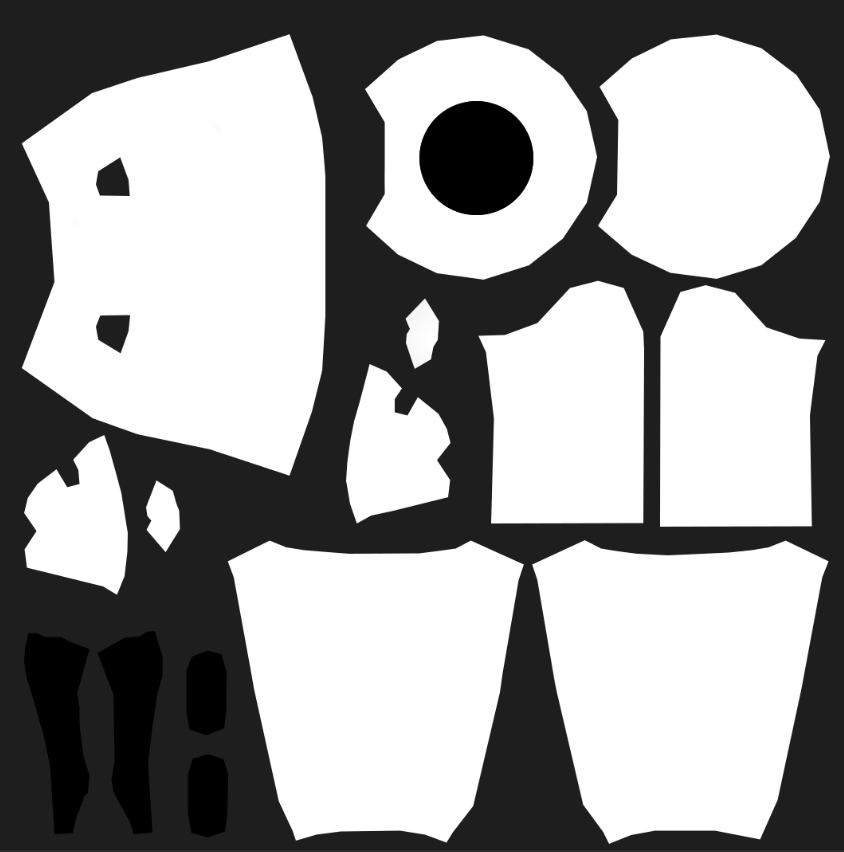
\includegraphics[width=0.8\textwidth]{chapters/theoretical_foundations/sections/models/resources/Texture.png}
        \caption{UV map}
        \label{fig:uv_map}
    \end{subfigure}
    \hfill
    \begin{subfigure}{0.45\textwidth}
        \centering
        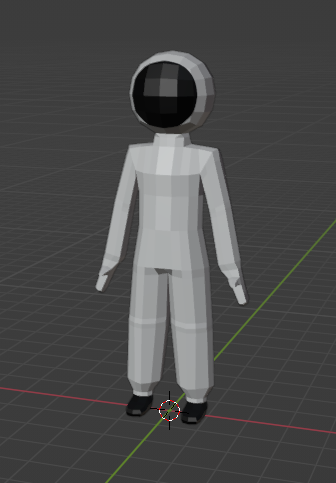
\includegraphics[width=0.8\textwidth]{chapters/theoretical_foundations/sections/models/resources/Model.png}
        \caption{Player model}
        \label{fig:player_model}
    \end{subfigure}

    \caption{Player model and the texture.}
\end{figure}
